\documentclass{article}
% \usepackage[utf8]{inputenc}
% \usepackage[T1]{fontenc}
\usepackage{algorithm2e}
\usepackage[pdftex]{graphicx}
\graphicspath{{images/}}
\DeclareGraphicsExtensions{.pdf,.png,.jpg}
\usepackage{amsmath}
\usepackage{mathtools}
\usepackage{booktabs}

\begin{document}



\newcommand{\add}[1]{{\text add}(#1)}
\newcommand{\rem}[1]{{\text rm}(#1)}

\newcommand{\motifs}{{\cal M}}
\newcommand{\motif}[1]{m_{#1}}

\newcommand{\mcount}{{\cal F}}
\newcommand{\mcountof}[1]{{\cal F}(\motif{#1})}
\newcommand{\mcountofat}[2]{{\cal F}_{#2}(\motif{#1})}



\newcommand{\ra}{$\rightarrow$}


\newcommand{\eqn}[1]{
	\begin{equation*}
		#1
	\end{equation*}
}

\newcommand{\eqna}[1]{
	\begin{eqnarray*}
		#1
	\end{eqnarray*}
}


% \newcommand{\operationAdd}[1]{add(\motif{#1})}
\newcommand{\operationAdd}[1]{+(#1)}
% \newcommand{\operationChange}[2]{change(\motif{#1},\motif{#2})}
\newcommand{\operationChange}[2]{(#1 \rightarrow #2)}

% \newcommand{\operationAddInv}[1]{add^{-1}(\motif{#1})}
\newcommand{\operationAddInv}[1]{-(#1)}
% \newcommand{\operationChangeInv}[2]{change^{-1}(\motif{#1},\motif{#2})}
\newcommand{\operationChangeInv}[2]{(#1 \leftarrow #2)}

\newcommand{\operation}{{\cal O}}
\newcommand{\signature}{{\cal S}}
\newcommand{\signatureofabcd}{\signature(a,b,c,d)}






\section{Counting motifs in dynamic graphs}
\label{sec:algorithm}

In this Secion, we describe basic insights regarding motifs in dynamic graphs.
Then, we describe \emph{StreaM}, a new stream-based algorithm for counting undirected 4-vertex motifs in dynamic graphs, and discuss its runtime complexity.






\subsubsection{Basic insights}

Whenever an edge $e = \{a,b\}$ is added to a graph $G_t$, i.e., update $u_{t+1} = add(e)$, two things happen: existing motifs are changed and new motifs are formed.
First, consider an existing motif $\motif{i}$ that consists of $a$, $b$, and $2$ other vertices.
The addition of $e$ causes the motif to change into a different motif $\motif{j}$ which contains one more edge.
We denote this operation as $\operationChange{i}{j}$.
Its execution decreases the occurrences of $\motif{i}$ and increases the occurrences of $\motif{j}$, i.e.,
\eqna{\operationChange{i}{j}:& \mcountofat{i}{t+1} := \mcountofat{i}{t} - 1,\; \mcountofat{j}{t+1} := \mcountofat{j}{t} + 1}
Second, consider vertices $c$ and $d$ that do not form a connected component with $a$ and $b$ without $e$'s existence.
In case $e$ connects the four vertices, a new motif $\motif{k}$ is formed.
We denote this operation as $\operationAdd{k}$.
Its execution increases the occurrences of $\motif{k}$, i.e.,
\eqna{\operationAdd{k}:& \mcountofat{k}{t+1} := \mcountofat{k}{t}+1}
In case an existing edge is removed, i.e., $u_{t+1} = rm(e)$, the inverse happens: some motifs are changed and others are dissolved.
We denote these operation as $\operationChange{i}{j}^{-1}$ and $\operationAdd{i}^{-1}$.
\eqna{\operationChange{i}{j}^{-1}:& \mcountofat{i}{t+1} := \mcountofat{i}{t} + 1,\; \mcountofat{j}{t+1} := \mcountofat{j}{t} - 1\\
\operationAdd{k}^{-1}:& \mcountofat{k}{t+1} := \mcountofat{k}{t}-1}
Adding or removing a vertex with degree 0 has no effect on the motif count.



\begin{figure}
\centering
  \centering
  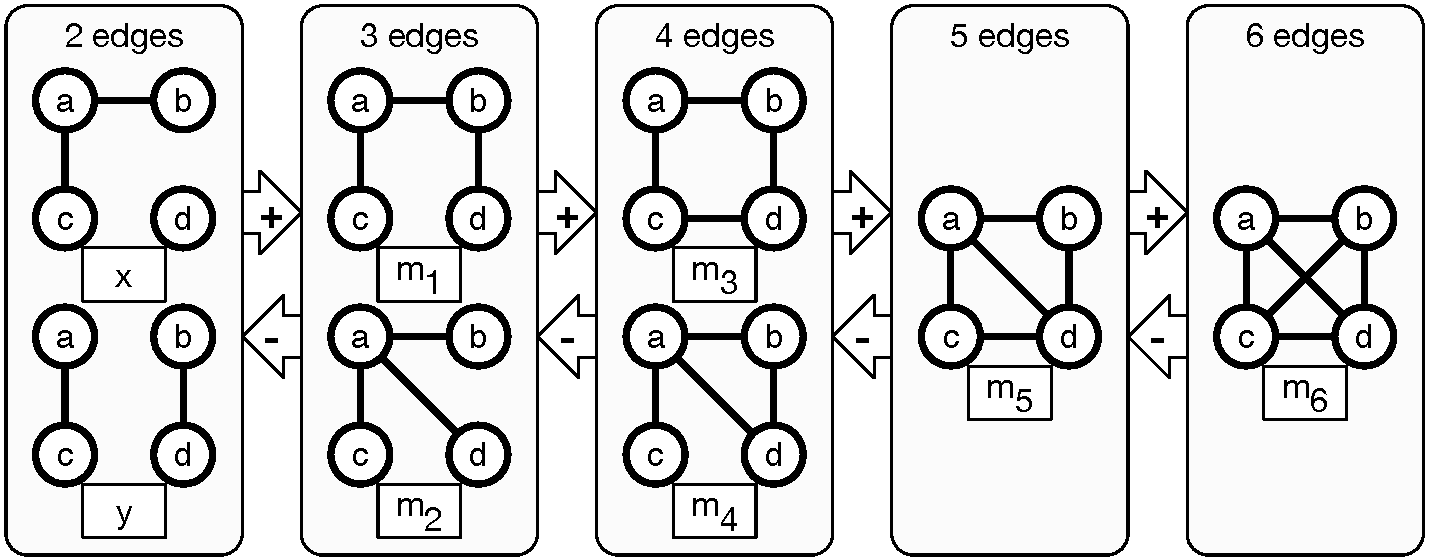
\includegraphics[width=1.0\textwidth]{idea-u}
  \caption{Transitions between the motifs $m_i \in \motifs$ when adding and removing edges}
  \label{fig:idea}
\end{figure}

Each motif $\motif{i} \in \motifs$ contains at least 3 and at most 6 edges.
The addition and removal of edges leads to transitions between them (cf. Figure~\ref{fig:idea}).
For example, adding the missing edge to $\motif{5}$ changes it to $\motif{6}$ ($\operationChange{5}{6}$) while removing any edge from $\motif{6}$ changes it to $\motif{5}$ ($\operationChange{5}{6}^{-1}$).
Adding edge $\{b,d\}$ to the disconnected set of nodes $x$ creates a new motif $\motif{1}$ ($\operationAdd{1}$) which is dissolved by the removal of any of its 3 edges ($\operationAdd{1}^{-1}$).

The main idea behind our new stream-based algorithm is to find and apply these operations to correctly update $\mcount$ for each edge addition and removal.
% occurring in the dynamic graph.
% Hence, we must find all motifs affected by an update and determine the respective operation.









\subsubsection{\emph{StreaM}}

% CD(a,b)
Assume an update (addition or removal) of edge $e=\{a,b\}$.
To correctly adapt $\mcount$, we need to consider all 2-vertex sets $\{c,d\} \in CD(a,b)$ such that $a$, $b$, $c$, and $d$ form a motif if $e$ exists.
Either both vertices are connected to $a$ or $b$ directly or $d$ is a neighbor of $c$ which is connected to $a$ or $b$.
With \eqn{N(a,b) := (n(a) \cup n(b)) \backslash \{a,b\},} we can define $CD(a,b)$ as follows:
\eqn{CD(a,b) = \{\{c,d\} : (c,d \in N(a,b), c \neq d) \lor (c \in N(a,b), d \in n(c) \backslash \{a,b\})\}}

% signature
Besides $\{a,b\}$, 5 edges are possible between $a$, $b$, $c$, and $d$.
We denote their existence as a quintuple $\signatureofabcd = (ac, ad, bc, bd, cd)$, called their \emph{signature}.
At least two distinct edges must exist, the first connecting $c$ and the second connecting $d$.
Therefore, there are $2^5 - 2 \cdot 2^2 = 24$ possible signatures.

\newcommand{\addImage}[3]{
	\includegraphics[width=0.07\textwidth]{u-operations/#2}
}
\newcommand{\addSignature}[3]{
	{\scriptsize
	\begin{tabular}[x]{@{}c@{}}
		#1
	\end{tabular}
	}
}
\newcommand{\addOperation}[3]{
	{\scriptsize $\operationAdd{#3}$ }
}
\newcommand{\changeImage}[4]{
	\includegraphics[width=0.07\textwidth]{u-operations/#2}
}
\newcommand{\changeSignature}[4]{
	{\scriptsize
	\begin{tabular}[x]{@{}c@{}}
		#1
	\end{tabular}
	}
}
\newcommand{\changeOperation}[4]{
	{\scriptsize $\operationChange{#3}{#4}$ }
}
\begin{table*}
\centering
\caption{Operation mapping $\operation$ from signatures $\signatureofabcd$ to operations}
\label{tab:operations}
\begin{tabular}{ccccccccccc}
	\toprule
	$\signature$ &
	\addSignature{10010\\01100}{1-ab}{1} &
	\addSignature{10001\\01001\\00101\\00011}{1-a}{1} &
	\addSignature{11000\\00110}{2}{2} &
	\addSignature{11001\\00111}{4}{4} &
	\changeSignature{10011\\01101}{1--3}{1}{3} &
	\changeSignature{11100\\11010\\10110\\01110}{1--4}{1}{4} &
	\changeSignature{10101\\01011}{2--4}{2}{4} &
	\changeSignature{11110}{3--5}{3}{5} &
	\changeSignature{11101\\11011\\10111\\01111}{4--5}{4}{5} &
	\changeSignature{11111}{5--6}{5}{6} \\
	\midrule
	$\operation$ &
	\addOperation{10 01 0\\01 10 0}{1-ab}{1} &
	\addOperation{10 00 1\\01 00 1\\00 10 1\\00 01 1}{1-a}{1} &
	\addOperation{11 00 0\\00 11 0}{2}{2} &
	\addOperation{11 00 1\\00 11 1}{4}{4} &
	\changeOperation{10 01 1\\01 10 1}{1--3}{1}{3} &
	\changeOperation{11 10 0\\11 01 0\\10 11 0\\01 11 0}{1--4}{1}{4} &
	\changeOperation{10 10 1\\01 01 1}{2--4}{2}{4} &
	\changeOperation{11 11 0}{3--5}{3}{5} &
	\changeOperation{11 10 1\\11 01 1\\10 11 1\\01 11 1}{4--5}{4}{5} &
	\changeOperation{11 11 1}{5--6}{5}{6} \\
	\midrule
	&
	\addImage{10 01 0\\01 10 0}{1-ab}{1} &
	\addImage{10 00 1\\01 00 1\\00 10 1\\00 01 1}{1-a}{1} &
	\addImage{11 00 0\\00 11 0}{2}{2} &
	\addImage{11 00 1\\00 11 1}{4}{4} &
	\changeImage{10 01 1\\01 10 1}{1--3}{1}{3} &
	\changeImage{11 10 0\\11 01 0\\10 11 0\\01 11 0}{1--4}{1}{4} &
	\changeImage{10 10 1\\01 01 1}{2--4}{2}{4} &
	\changeImage{11 11 0}{3--5}{3}{5} &
	\changeImage{11 10 1\\11 01 1\\10 11 1\\01 11 1}{4--5}{4}{5} &
	\changeImage{11 11 1}{5--6}{5}{6} \\
	\bottomrule
\end{tabular}
\end{table*}








% \begin{table*}
% \centering
% \caption{XXXX Operation mapping $\operation$ from signatures $\signatureofabcd$ to operations}
% \label{tab:operationsX}
% \begin{tabular}{cccccc}
% 	\toprule
% 	% $\signature$ &
% 	% \addSignature{10010\\01100}{1-ab}{1} &
% 	% \addSignature{10001\\01001\\00101\\00011}{1-a}{1} &
% 	% \addSignature{11000\\00110}{2}{2} &
% 	% \addSignature{11001\\00111}{4}{4} &
% 	% \changeSignature{10011\\01101}{1--3}{1}{3} \\
% 	% \midrule
% 	$\operation$ &
% 	\addOperation{10 01 0\\01 10 0}{1-ab}{1} &
% 	\addOperation{10 00 1\\01 00 1\\00 10 1\\00 01 1}{1-a}{1} &
% 	\addOperation{11 00 0\\00 11 0}{2}{2} &
% 	\addOperation{11 00 1\\00 11 1}{4}{4} &
% 	\changeOperation{10 01 1\\01 10 1}{1--3}{1}{3} \\
% 	\midrule
% 	&
% 	\addImage{10 01 0\\01 10 0}{1-ab}{1} &
% 	\addImage{10 00 1\\01 00 1\\00 10 1\\00 01 1}{1-a}{1} &
% 	\addImage{11 00 0\\00 11 0}{2}{2} &
% 	\addImage{11 00 1\\00 11 1}{4}{4} &
% 	\changeImage{10 01 1\\01 10 1}{1--3}{1}{3} \\
% 	% \midrule
% 	% $\signature$ &
% 	% \changeSignature{11100\\11010\\10110\\01110}{1--4}{1}{4} &
% 	% \changeSignature{10101\\01011}{2--4}{2}{4} &
% 	% \changeSignature{11110}{3--5}{3}{5} &
% 	% \changeSignature{11101\\11011\\10111\\01111}{4--5}{4}{5} &
% 	% \changeSignature{11111}{5--6}{5}{6} \\
% 	\midrule
% 	$\operation$ &
% 	\changeOperation{11 10 0\\11 01 0\\10 11 0\\01 11 0}{1--4}{1}{4} &
% 	\changeOperation{10 10 1\\01 01 1}{2--4}{2}{4} &
% 	\changeOperation{11 11 0}{3--5}{3}{5} &
% 	\changeOperation{11 10 1\\11 01 1\\10 11 1\\01 11 1}{4--5}{4}{5} &
% 	\changeOperation{11 11 1}{5--6}{5}{6} \\
% 	\midrule
% 	&
% 	\changeImage{11 10 0\\11 01 0\\10 11 0\\01 11 0}{1--4}{1}{4} &
% 	\changeImage{10 10 1\\01 01 1}{2--4}{2}{4} &
% 	\changeImage{11 11 0}{3--5}{3}{5} &
% 	\changeImage{11 10 1\\11 01 1\\10 11 1\\01 11 1}{4--5}{4}{5} &
% 	\changeImage{11 11 1}{5--6}{5}{6} \\
% 	\bottomrule
% \end{tabular}
% \end{table*}










% operations
Each signature corresponds to a specific operation that must be executed to update $\mcount$.
 % to account for the addition (or removal) of $\{a,b\}$.
We define a function $\operation$ that maps a signature $\signature$ on the corresponding operation.
The complete assignment of signatures to operations is given in Table~\ref{tab:operations}.
In case the edge $\{a,b\}$ is removed instead of added, the inverse operation must be executed.
As an example consider the signature $(10010)$ which is isomorph to $(01100)$.
The addition of $\{a,b\}$ creates the motif $\motif{1}$.
Its removal dissolves the motif as $a$, $b$, $c$, and $d$ are no longer connected.

% algorithm
Based on $\signature$ and $\operation$, we can now describe the stream-based algorithm \emph{StreaM} for updating the motif frequency in an undirected graph (cf. Algorithm~\ref{alg:u}).
For an edge $\{a,b\}$ that is added or removed (described by $type$), we first determine the set $CD(a,b)$ of all pairs of vertices connected to $a$ and $b$.
For each pair $\{c,d\} \in CD(a,b)$, the required operation $o = \operation(\signatureofabcd)$ is determined from the signature of $a$, $b$, $c$, and $d$.
If $\{a,b\}$ is added, the operation $o$ is executed.
Otherwise, the inverse operation $o^{-1}$ is executed.

\begin{algorithm}[!htb]
	\KwData{$G, \{a,b\}, type \in \{add, rm\}$}
	\SetKwComment{Comment}{/* }{ */}
	\Begin{
		\For{$\{c,d\} \in CD(a,b)$}{
			$o = \operation(\signatureofabcd)$ \Comment*[r]{operation}
			\uIf{$type = add$}{
				execute $o$ \Comment*[r]{edge is added}
			}
      		\uElseIf{$type = rm$}{
       			 execute $o^{-1}$ \Comment*[r]{edge is removed}
			}
		}
	}
	\caption{\emph{StreaM} for maintaining $\mcount$ in dynamic graphs}
	\label{alg:u}
\end{algorithm}





\subsubsection{Complexity discussion}

\emph{StreaM} iterates over the $|CD(a,b)| \leq 5 \cdot (d_{max})^2$ elements of $CD(a,b)$.
For each element $\{c,d\}$, it computes the signature which can be done in $5 \cdot O(1)$ time, assuming hash-based datastructures are used for adjacency lists.
In addition, $\mcount$ is incremented or decremented which has time complexity of $O(1)$ as well.
Therefore, processing a single edge addition or removal with \emph{StreaM} has time complexity of
\eqn{O((d_{max})^2) \cdot (O(1) + O(1)) = O((d_{max})^2)}



\end{document}